\documentclass[a4paper,fontsize=12pt]{article}
\usepackage{fontspec}                 % loaded by polyglossia, but included here for transparency
\usepackage{polyglossia}
\usepackage{indentfirst}              % Insert "Red line"

\setmainlanguage{russian}
\setotherlanguage{english}

\usepackage{graphicx}         % Insert images
\usepackage{siunitx}          % for \ang macros
\usepackage{units}            % for fraction with unit
\usepackage{wasysym}          % for \diameter


\newfontfamily\russianfont[Script=Cyrillic]{Arial}

% \setlength{\tabcolsep}{2pt}

\usepackage[left=3.5cm,right=2cm,top=2.5cm,bottom=2.5cm,bindingoffset=0cm]{geometry}
% XeLaTeX can use any font installed in your system fonts folder
% Linux Libertine in the next line can be replaced with any
% OpenType or TrueType font that supports the Cyrillic script.

\begin{document}

\begin{titlepage}
  \thispagestyle{empty}

  \begin{center}
    \Large{\textbf{Национальный исследовательский университет МИЭТ}}

    \vspace{5cm}

    \huge{\textbf{\textit{Расчетно-графическая работа}}}

    \large{по дисциплине}

    \large{«Метрология, стандартизация и сертификация»}

    \vspace{5cm}

    \huge{\textbf{\textit{«Анализ точных сопряжений в узле»}}}
  \end{center}

  \vspace{1cm}

  \begin{flushright}
    \textbf{Выполнил:}                  \linebreak
    Студент группы ЭКТ-26               \linebreak
    Чечетин П. Е.                       \linebreak
  \end{flushright}

  \vfill

  \begin{center}
    \Large{Москва – 2013}
  \end{center}
\end{titlepage}

\newpage

\tableofcontents

\newpage


\section{Вариант}

\resizebox{14cm}{!} {
  \begin{tabular}{ |l*{10}{|c}| }
  \hline
  \multicolumn{5}{|c}{Диаметральные размеры} & \multicolumn{5}{|c|}{Осевые размеры} \\
  \hline
  d1        & d2      & d3      & d4        & d5        & L   & l1  & l2 & l3 & l4 \\
  \hline
  9js7	    & 10e10	  & 10L0-k7	& 10F9-k7	  & 9H8-js7	  & 88	& 14	& 25 & 65 & 18 \\
  \hline
  \end{tabular}
}

\section{Эскиз детали}

\begin{figure}[h]
    \centering
    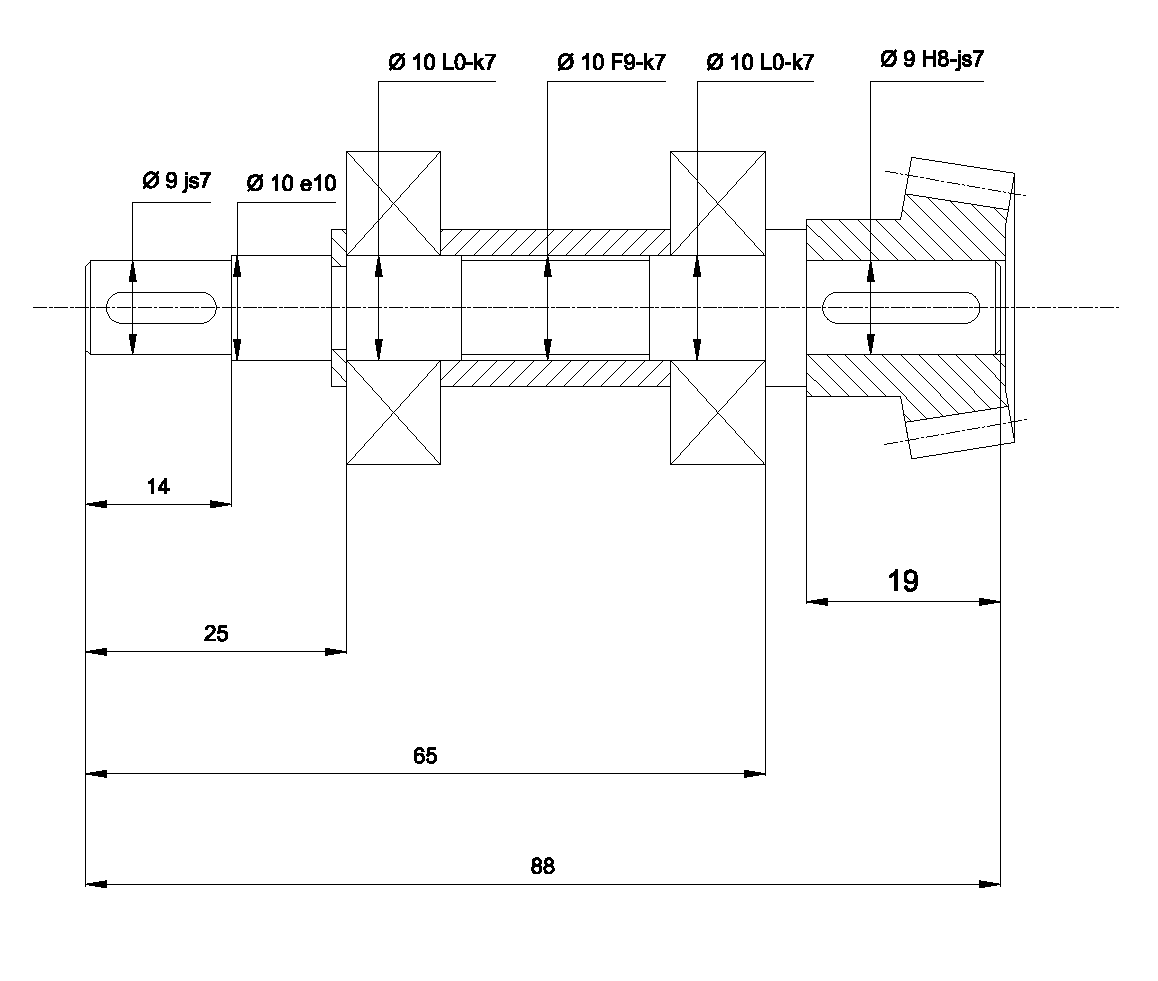
\includegraphics[width=16cm]{images/draw1.eps}
    % Angular distribution of sputtered atoms (dashed) and reflected ions (solid) compared to a cosine distribution (circle) for incidence angles of 0°, 40°, 70° and 87°.
    \label{fig:draw1}
\end{figure}

\newpage
\section{Определение предельных отклонений на диаметральные размеры}

\subsection{Вал $d_1$: \diameter 9.0 js7}
es = 7 мкм

ei = -7 мкм

$d_{1max}$ = $d_{1H}$ + es = 9 + 0.007 = 9.007 мм

$d_{1min}$ = $d_{1H}$ + ei = 9 - 0.007 = 8.887 мм

\subsection{Вал $d_2$: \diameter 10 e10}
es = -25 мкм

ei = -83 мкм

$d_{2max}$ = $d_{2H}$ + es = 10 - 0.025 = 9.975 мм

$d_{2min}$ = $d_{2H}$ + ei = 10 - 0.083 = 9.917 мм

\subsection{Сопряжение $d_3$: \diameter 10 L0-k7}
ES = 0 мкм

EI = -8 мкм

es = 16 мкм

ei = 1 мкм

$D_{3max}$ = $D_{3H}$ + ES = 10 + 0 = 10 мм

$D_{3min}$ = $D_{3H}$ + EI = 10 - 0.008 = 9.992 мм

$d_{3max}$ = $d_{3H}$ + es = 10 + 0.016 = 10.016 мм

$d_{3min}$ = $d_{3H}$ + ei = 10 + 0.001 = 10.001 мм

$S_{3max}$ = ES - es = 0 - 16 = -16 мкм

$S_{3min}$ = EI - ei = -8 - 1 = -9 мкм

$S_{3m}$ = $\frac{S_{3max} + S_{3min}}{2}$ = -12.5 мкм

\textbf{Посадка подшипниковая, c натягом}

\subsection{Сопряжение $d_4$: \diameter 10 F9-k7}
ES = 49 мкм

EI = 13 мкм

es = 16 мкм

ei = 1 мкм

$D_{4max}$ = $D_{4H}$ + ES = 10 + 0.049 = 10.049 мм

$D_{4min}$ = $D_{4H}$ + EI = 10 + 0.013 = 10.013 мм

$d_{4max}$ = $d_{4H}$ + es = 10 + 0.016 = 10.016 мм

$d_{4min}$ = $d_{4H}$ + ei = 10 + 0.001 = 10.001 мм

$S_{4max}$ = ES - es = 49 - 16 = 33 мкм

$S_{4min}$ = EI - ei = 13 - 1 = 12 мкм

$S_{4m}$ = $\frac{S_{4max} + S_{4min}}{2}$ = 22.5 мкм

\textbf{Посадка переходная с преобладанием зазора}

\subsection{Сопряжение $d_5$: \diameter 9 H8-js7}
ES = 22 мкм

EI = 0 мкм

es = 7 мкм

ei = -7 мкм

$D_{5max}$ = $D_{5H}$ + ES = 9 + 0.022 = 9.022 мм

$D_{5min}$ = $D_{5H}$ + EI = 9 - 0 = 9 мм

$d_{5max}$ = $d_{5H}$ + es = 9 + 0.007= 9.007 мм

$d_{5min}$ = $d_{5H}$ + ei = 9 - 0.007 = 8.993 мм

$S_{5max}$ = ES - es = 22 - 7 = 15 мкм

$S_{5min}$ = EI - ei = 0 + 7 = 7 мкм

$S_{5m}$ = $\frac{S_{5max} + S_{5min}}{3}$ = 11 мкм

\textbf{Посадка в системе основного отверстия преобладанием зазора}

\subsection{Схема допусков}
\begin{figure}[h]
    \centering
    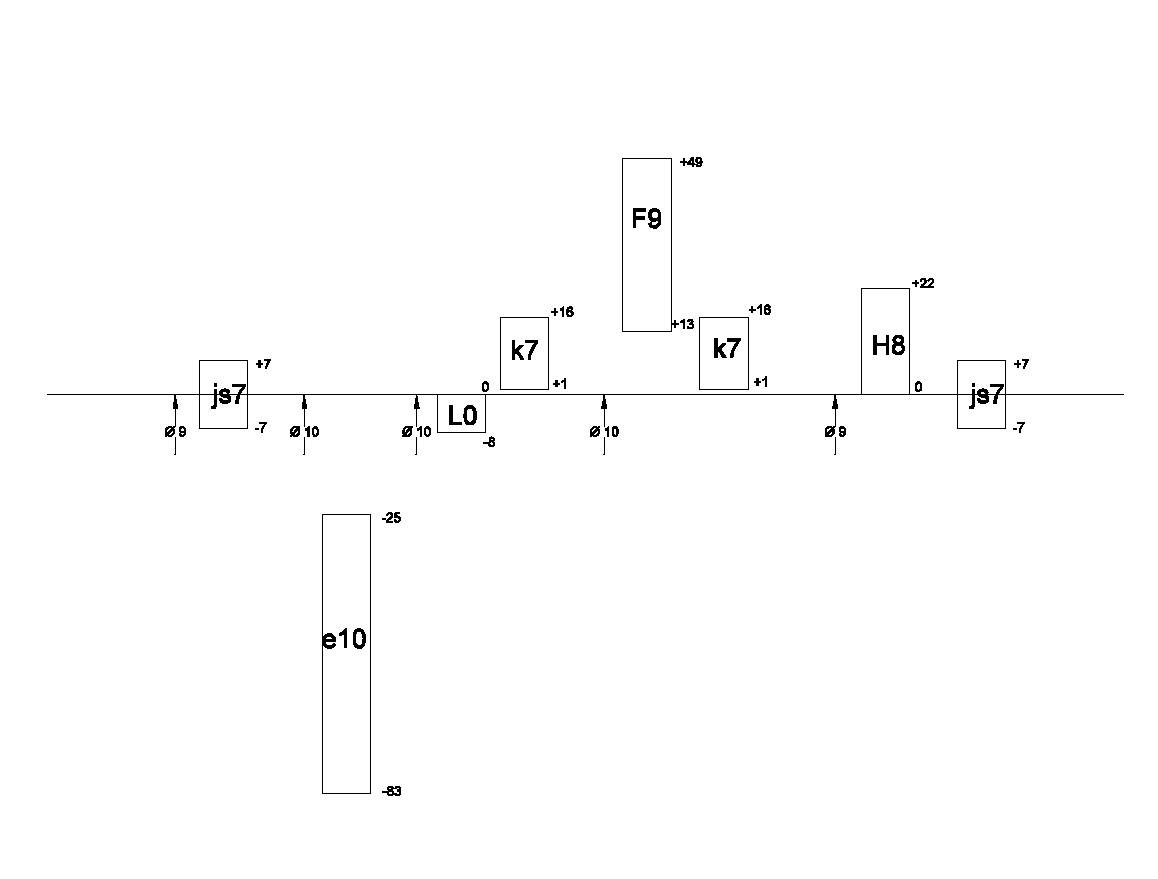
\includegraphics[width=16cm]{images/draw3.eps}
    \label{fig:draw}
\end{figure}


\section{Определение параметров шероховатости}

\subsection{Вал $d_1$: \diameter 9.0 js7}

$T_d = es - ei = 0.007 + 0.007 = 0.014$ мм

$R_z \leq 0.3 * T_d \equiv R_z \leq 4.2$

$R_z = 3.2$

$R_a = 0.63$

\subsection{Вал $d_2$: \diameter 10 e10}
$T_d = es - ei = -25 - 83 = 0.058$ мм

$R_z \leq 0.3 * T_d \equiv R_z \leq 17.4$

$R_z = 10$

$R_a = 2.5$

\subsection{Сопряжение $d_3$: \diameter 10 L0-k7}
$T_d = es - ei = 0.016 - 0.001 = 0.015$ мм

$R_z \leq 0.3 * T_d \equiv R_z \leq 4.5$

$R_z = 3.2$

$R_a = 0.63$


\subsection{Сопряжение $d_4$: \diameter 10 F9-k7}
$T_d = es - ei = 0.016 - 0.001 = 0.015$ мм

$R_z \leq 0.3 * T_d \equiv R_z \leq 4.5$

$R_z = 3.2$

$R_a = 0.63$

\subsection{Сопряжение $d_5$: \diameter 9 H8-js7}
$T_d = es - ei = 0.007 + 0.007 = 0.014$ мм

$R_z \leq 0.3 * T_d \equiv R_z \leq 4.2$

$R_z = 3.2$

$R_a = 0.63$

\newpage
\section{Эскиз вала}

\begin{figure}[h]
    \centering
    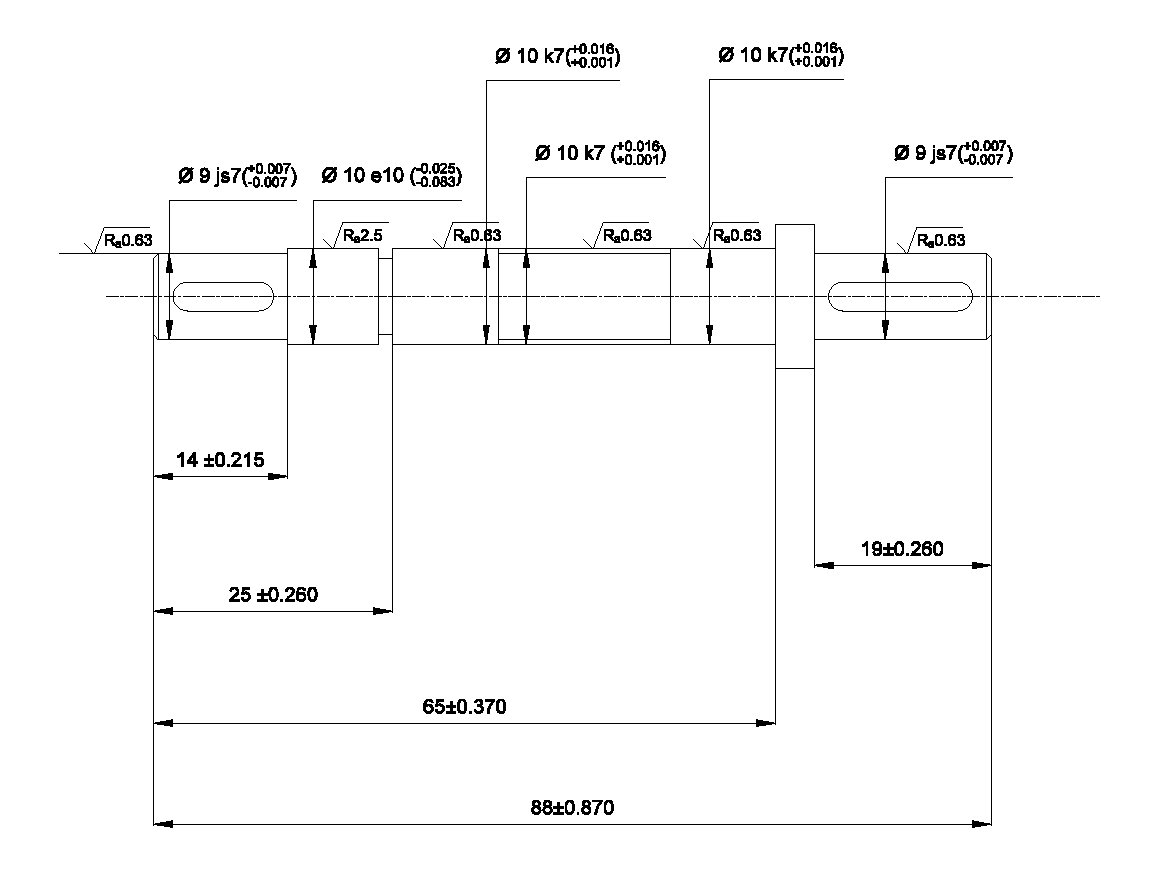
\includegraphics[width=16cm]{images/draw2.eps}
    \label{fig:draw2}
\end{figure}


\end{document}

